%Version 3 October 2023
% See section 11 of the User Manual for version history
%
%%%%%%%%%%%%%%%%%%%%%%%%%%%%%%%%%%%%%%%%%%%%%%%%%%%%%%%%%%%%%%%%%%%%%%
%%                                                                 %%
%% Please do not use \input{...} to include other tex files.       %%
%% Submit your LaTeX manuscript as one .tex document.              %%
%%                                                                 %%
%% All additional figures and files should be attached             %%
%% separately and not embedded in the \TeX\ document itself.       %%
%%                                                                 %%
%%%%%%%%%%%%%%%%%%%%%%%%%%%%%%%%%%%%%%%%%%%%%%%%%%%%%%%%%%%%%%%%%%%%%

%%\documentclass[referee,sn-basic]{sn-jnl}% referee option is meant for double line spacing

%%=======================================================%%
%% to print line numbers in the margin use lineno option %%
%%=======================================================%%

%%\documentclass[lineno,sn-basic]{sn-jnl}% Basic Springer Nature Reference Style/Chemistry Reference Style

%%======================================================%%
%% to compile with pdflatex/xelatex use pdflatex option %%
%%======================================================%%

%%\documentclass[pdflatex,sn-basic]{sn-jnl}% Basic Springer Nature Reference Style/Chemistry Reference Style


%%Note: the following reference styles support Namedate and Numbered referencing. By default the style follows the most common style. To switch between the options you can add or remove “Numbered” in the optional parenthesis. 
%%The option is available for: sn-basic.bst, sn-vancouver.bst, sn-chicago.bst%  
 
%%\documentclass[sn-nature]{sn-jnl}% Style for submissions to Nature Portfolio journals
%%\documentclass[sn-basic]{sn-jnl}% Basic Springer Nature Reference Style/Chemistry Reference Style
\documentclass[sn-mathphys-num]{sn-jnl}% Math and Physical Sciences Numbered Reference Style 
%%\documentclass[sn-mathphys-ay]{sn-jnl}% Math and Physical Sciences Author Year Reference Style
%%\documentclass[sn-aps]{sn-jnl}% American Physical Society (APS) Reference Style
%%\documentclass[sn-vancouver,Numbered]{sn-jnl}% Vancouver Reference Style
%%\documentclass[sn-apa]{sn-jnl}% APA Reference Style 
%%\documentclass[sn-chicago]{sn-jnl}% Chicago-based Humanities Reference Style

%%%% Standard Packages
%%<additional latex packages if required can be included here>

\newcommand{\ra}[1]{\renewcommand{\arraystretch}{#1}}
\usepackage{tabularx}
\usepackage[table]{xcolor}
\usepackage{graphicx}
\usepackage{multirow}
\usepackage{amsmath,amssymb,amsfonts}%
\usepackage{amsthm}%
\usepackage{mathrsfs}%
\usepackage[title]{appendix}%
\usepackage{xcolor}%
\usepackage{textcomp}%
\usepackage{manyfoot}%
\usepackage{booktabs}
\usepackage{algorithm}%
\usepackage{algorithmicx}%
\usepackage{algpseudocode}%
\usepackage{listings}%
\usepackage{multicol}
\usepackage[export]{adjustbox}

\usepackage{comment}
\usepackage{float}
%%%%

%%%%%=============================================================================%%%%
%%%%  Remarks: This template is provided to aid authors with the preparation
%%%%  of original research articles intended for submission to journals published 
%%%%  by Springer Nature. The guidance has been prepared in partnership with 
%%%%  production teams to conform to Springer Nature technical requirements. 
%%%%  Editorial and presentation requirements differ among journal portfolios and 
%%%%  research disciplines. You may find sections in this template are irrelevant 
%%%%  to your work and are empowered to omit any such section if allowed by the 
%%%%  journal you intend to submit to. The submission guidelines and policies 
%%%%  of the journal take precedence. A detailed User Manual is available in the 
%%%%  template package for technical guidance.
%%%%%=============================================================================%%%%

%% as per the requirement new theorem styles can be included as shown below
\theoremstyle{thmstyleone}%
\newtheorem{theorem}{Theorem}%  meant for continuous numbers
%%\newtheorem{theorem}{Theorem}[section]% meant for sectionwise numbers
%% optional argument [theorem] produces theorem numbering sequence instead of independent numbers for Proposition
\newtheorem{proposition}[theorem]{Proposition}% 
%%\newtheorem{proposition}{Proposition}% to get separate numbers for theorem and proposition etc.

\theoremstyle{thmstyletwo}%
\newtheorem{example}{Example}%
\newtheorem{remark}{Remark}%

\theoremstyle{thmstylethree}%
\newtheorem{definition}{Definition}%

\raggedbottom
%%\unnumbered% uncomment this for unnumbered level heads

\begin{document}

\title[MiCSS: A Microsimulation Model for Colorectal Cancer Screening]{MiCSS: A Microsimulation Model for Colorectal Cancer Screening}

%%=============================================================%%
%% GivenName	-> \fnm{Joergen W.}
%% Particle	-> \spfx{van der} -> surname prefix
%% FamilyName	-> \sur{Ploeg}
%% Suffix	-> \sfx{IV}
%% \author*[1,2]{\fnm{Joergen W.} \spfx{van der} \sur{Ploeg} 
%%  \sfx{IV}}\email{iauthor@gmail.com}
%%=============================================================%%

\author[1]{\fnm{Tomás} \sur{Álvarez}\email{toalvarez@uc.cl}}

\author[1]{\fnm{Jorge} \sur{Vera}}\email{jver@uc.cl}
%\equalcont{These authors contributed equally to this work.}

\author[1,2]{\fnm{Diego} \sur{Rojas}}\email{dfrojas2@uc.cl}
%\equalcont{These authors contributed equally to this work.}

\author[3]{\fnm{Ricardo} \sur{Ahumada}}\email{r\_ahumada@uchile.cl}
%\equalcont{These authors contributed equally to this work.}

\author[3]{\fnm{Gloria} \sur{Stephens}}\email{gloria.stephens@ssms.gob.cl}



\affil[1]{\orgdiv{Department of Industrial Engineering and Systems}, \orgname{Pontificia Universidad Católica de Chile}, \orgaddress{\street{Avda. Vicuña Mackenna 4860}, \city{Santiago}, \postcode{7820436}, \state{Región Metropolitana}, \country{Chile}}}

\affil[2]{\orgdiv{Information Technologies}, \orgname{National Cancer Institute}, \orgaddress{\street{Av. Profesor Zañartu 1010}, \city{Santiago}, \postcode{8380455}, \state{Región Metropolitana}, \country{Chile}}}

\affil[3]{\orgdiv{Management and Networks Department}, \orgname{Southern Metropolitan Health Service}, \orgaddress{\street{Av. Santa Rosa 3453}, \city{Santiago}, \postcode{8900390}, \state{Región Metropolitana}, \country{Chile}}}

%%================================%%
%% Sample for structured abstract %%
%%================================%%

\abstract{\textbf{Purpose:} This study presents the MiCSS microsimulation model. An open source model set to analyze the cost effectiveness of implementing a colorectal cancer (CRC) screening strategy considering all the individuals of a population.

\textbf{Methods:} The model simulates a screening strategy that consists on performing fecal immunochemical tests (FIT) on individuals of the population who adhere to the strategy and are within the selected age interval. CRC detection occurs either asymptomatically through the screening test or symptomatically when individuals present with symptoms at a healthcare facility. The success of the screening strategy is measured in its ability to detect CRC in its asymptomatic stage. All parameters were adjusted to the values recommended by the medical community. The results were obtained using demographic data from the southern district of Santiago, Chile.
 
\textbf{Results:} The scenarios presented use the proposed values for all parameters except for population adherence, which varies from 0\% to 80\%. As population adherence increases, the prognosis for CRC patients improves, but overall costs also rise. The cost of biennial FIT strategies at adherence rates above 0\% ranged from as high as 6,348 USD per DALY to as low as 4,479 USD per DALY. At 80\% adherence, the number of necessary yearly FITs and colonoscopies would be 141,707 and 8,843, respectively. Probabilistic sensitivity analysis (1,000 iterations) confirms that screening is cost-effective in over 96\% of iterations at standard willingness-to-pay thresholds.
 
\textbf{Conclusion:} The simulation model was successful at delivering the cost effectiveness of implementing a screening strategy for CRC in this region. Both deterministic and probabilistic analyses confirm that biennial FIT screening is robustly cost-effective. The model is publicly available for anyone to utilize and improve upon.
}
\keywords{microsimulation, healthcare, screening, colorectal cancer}

%%\pacs[JEL Classification]{D8, H51}

%%\pacs[MSC Classification]{35A01, 65L10, 65L12, 65L20, 65L70}

\maketitle

\section*{Context}

\begin{itemize}
    \item \textbf{Key Objective:} Introducing a model that analyzes the cost effectiveness of implementing a colorectal cancer (CRC) screening strategy in a specific region.

    \item \textbf{Knowledge Generated:} A new publicly available microsimulation model that facilitates the cost-effectiveness analysis of implementing a CRC screening strategy, written in Python, validated following the Eddy et al.\ (2012) five-type framework, and evaluated with both deterministic and probabilistic sensitivity analyses.

    \item \textbf{Relevance:} Screening strategies for CRC and other cancers have been shown to improve prognosis. This new model gives access to policymakers to make evidence-based decisions regarding the implementation of such strategies.
\end{itemize}

\section{Introduction}\label{sec1}

% Definition of Micro-Simulation Models (MSMs)
Micro-Simulation Models (MSMs) are a technique which use individual level data or units to model economic and social outcomes. By focusing on individual agents, MSMs provide detailed insights into the distributional effects of interventions, allowing for a nuanced understanding of policy impacts. MSMs have evolved to address the challenges of detailed and large-scale simulations, with innovations making them increasingly flexible and applicable to public policy analysis \cite{klevmarken_microsimulation_2022}. 

% Benefits of MSMs in disease simulation:
MSMs offer significant advantages over traditional models, especially in disease simulation. They integrate observed data from diverse sources, such as government databases, clinical trials, and expert opinions, directly into the simulation. This flexibility and scalability make MSMs one of the most effective tools for modeling the progression of chronic diseases. One of the key benefits is their focus on individual patients rather than averages. This allows for personalized data, such as birth year, comorbidities, and disease characteristics, to be incorporated for each simulated individual \cite{chrysanthopoulou_milc_2016}.

% Challenges of MSM Development:
Developing a MSM presents multiple challenges, particularly related to data quality, budget, and project management. Reliable models require accurate data, which is often incomplete or difficult to obtain. Additionally, building a model fit for policy analysis involves significant financial resources, sometimes amounting to millions of dollars, and requires years of collaboration from interdisciplinary teams. Effective project management is essential to prevent budget overruns and delays. Furthermore, aligning MSM outputs with macro-level projections is crucial to ensure the accuracy and policy relevance of the results \cite{harding_challenges_2023}.

% Examples of MSMs in Colon Cancer Research:
MSMs were first theorized by Guy Orcutt in 1957, with the first model published in 1961 \cite{orcutt_new_1957, orcutt_microanalysis_1963}. In 1985, the MISCAN model was developed to evaluate mass disease screening \cite{habbema_miscan_1985}, which later inspired the MISCAN-Colon model, specific to colorectal cancer \cite{loeve_miscan-colon_1999}. MISCAN-Colon continues to be widely used today \cite{van_den_puttelaar_effectiveness_2024}, showcasing the long-term adaptability of MSMs. The model’s ability to remain accurate through updates over the years highlights the enduring value of MSMs in healthcare research \cite{gini_development_2021}.

% Introduction to the MiCSS Model:
The Micro Colorectal Cancer Screening Simulator (MiCSS) is a new, dynamic, discrete time microsimulation model programmed entirely in Python. The model simulates individual life trajectories, both for those with and without colorectal cancer (CRC), by incorporating events that can change their health status. Every individual in the model faces eventual death, which can occur from CRC or other causes. For those who adhere to the screening process, screening events are incorporated into their life trajectories. In cases where CRC develops, the disease initially manifests asymptomatically, with symptoms appearing years later. The primary goal of the screening process is to detect cases during this asymptomatic stage, improving early detection and thus enhancing prognosis and treatment outcomes for CRC patients.

% Reason behind the creation of MiCSS:
The main reason for the creation of MiCSS was the unavailability of open source colorectal cancer screening models. Currently, most, if not all, simulation models for CRC screening are not accessible without request. Furthermore, they are written in old and hard to understand programming languages like Delphi(MISCAN-Colon), C(SimCRC) or C\#(CRC-SPIN) \cite{noauthor_miscan-colon_nodate,noauthor_simcrc_nodate, noauthor_crc-spin_nodate}. The MiCSS model is publicly available in a repository for anyone to use and improve upon. It is written in the Python language, which allows a large number of individuals to understand it, critique it and hopefully improve it.

% Purpose of MiCSS:
Recent studies emphasize the importance of preventive medicine in CRC care, recommending the implementation of screening strategies to improve prognosis \cite{hossain_colorectal_2022, baidoun_colorectal_2021, rawla_epidemiology_2019, van_rossum_earlier_2009, soerjomataram_most_2012}. While some countries have successfully implemented screening strategies, most have yet to implement public policies for this endeavor \cite{navarro_colorectal_2017}. The idea behind the creation of MiCSS is to allow anyone to evaluate the cost effectiveness of implementing a CRC screening strategy in their own region.

% What this paper is about
This article introduces the MiCSS model in its first iteration, describing its components, algorithm and sources of data. It also presents the results of the use of this model on the southern region of Santiago of Chile. Finally, the relevance, outcomes and challenges of this model are discussed, describing the future work needed to validate it in the CRC research community.

\section{Methods}

The MiCSS model consists of two independent components. The first component are the individuals within the studied population, while the second is the data collected over time as the screening strategy is applied to this population.

\subsection{Model individuals}


% How individuals are created in the model
The moment each individuals enters the simulation, their set of characteristics and the ages at which they will experience health status changes are instantly defined.

First, key attributes such as year of birth, gender, age, and whether they will develop CRC are determined. Next, the specific ages at which health status changes will occur are calculated. These calculations are influenced by individual characteristics; for example, life expectancy is adjusted based on the person's year of birth and age.

\begin{figure}[H]
    \centering
    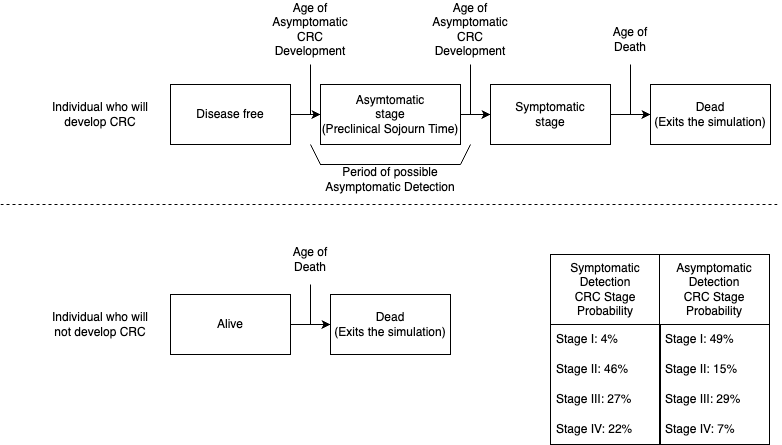
\includegraphics[width=1\textwidth]{images/MiCSSDiagram.png}
    \caption{Events for an Individual in the MiCSS Model}
    \label{fig:micss_diagram}
\end{figure}

The events for individuals in the simulation are illustrated in Figure \ref{fig:micss_diagram}. For individuals who develop CRC, the key events include the point at which the disease becomes detectable by screening tests, when it would be identified without preventive screening, and the moment of death due to the disease. In contrast, for individuals who do not develop CRC, the only event considered is death from other causes.

\subsubsection{CRC and non CRC individuals}
% On the separation of those with CRC and no CRC
The separation between individuals who will develop CRC or not is determined by the lifetime risk of developing CRC. The value used for this scenario is 4.2\%, which was obtained from the American Cancer Society \cite{noauthor_colorectal_nodate-1}. This means that non-CRC individuals account for approximately 95.8\% of the population.

CRC individuals have two simultaneous cancer stages assigned to them according to the symptomatic or asymptomatic detection of the disease. This means that, if the screening is not successful at detecting the disease, the cancer will have the symptomatic case cancer stage. The other scenario is in which the disease is detected asymptomatically thanks to the screening test, then the individual will have the asymptomatic case cancer stage. On average, individuals should get an earlier stage of cancer in their asymptomatic detection scenario than on the symptomatic one. In the case of a successful asymptomatic detection, the life expectancy of the individual is recalculated with their asymptomatic cancer stage. 

Screening significantly reduces the incidence of CRC by removing precancerous lesions during the colonoscopy procedure. A systematic review by Zhang et al.\ reported that CRC incidence is reduced by 52\% through this practice \cite{zhang_colonoscopic_2020}. The model incorporates this benefit: when a screening-detected cancer is found asymptomatically (true positive on FIT followed by colonoscopy), there is a 52\% probability that the lesion is reclassified as a removed polyp (polypectomy). In these cases, the individual's death age reverts to their natural (non-cancer) lifespan, no cancer treatment cost is incurred beyond the colonoscopy itself, and the individual is no longer counted as a cancer death. The remaining 48\% of screening-detected cancers proceed with asymptomatic-stage treatment as before.

Individuals who will not develop CRC have their own life expectancy calculation, which is done using their year of birth and age.

\subsubsection{Screening}

For this model, the screening exam utilized is the fecal immunochemical test (FIT), which is the recommended test for CRC screening \cite{zhu_comparison_2010}.

The screening is heavily dependent on two parameters: sensitivity and specificity. The sensitivity of a test refers to its ability to accurately detect true positives, meaning it correctly identifies all individuals who have a condition. Contrariwise, the specificity of a test measures its ability to accurately detect true negatives, meaning it correctly identifies individuals who do not have a condition.

According to a meta study by Lee et al. the sensitivity and specificity of FIT exams is 79\% and 94\% respectively. Screening is conducted on individuals within age ranges where CRC cases are most prevalent, influenced by the duration of the asymptomatic stage and test precision. Following the recommendations of the American College of Physicians, ages of CRC cases and sojourn time of the asymptomatic stage, the screening is set for ages 50 to 75, with a biennial frequency \cite{noauthor_colorectal_nodate-1, noauthor_uscs_2024, brenner_sojourn_2011}.

A critical consequence of these parameters is that approximately 6\% of individuals without CRC—who make up 95.8\% of those tested—will yield a false positive result, necessitating follow-up colonoscopies that confirm the absence of CRC.



\begin{center}
\begin{figure}[H]
    \centering
    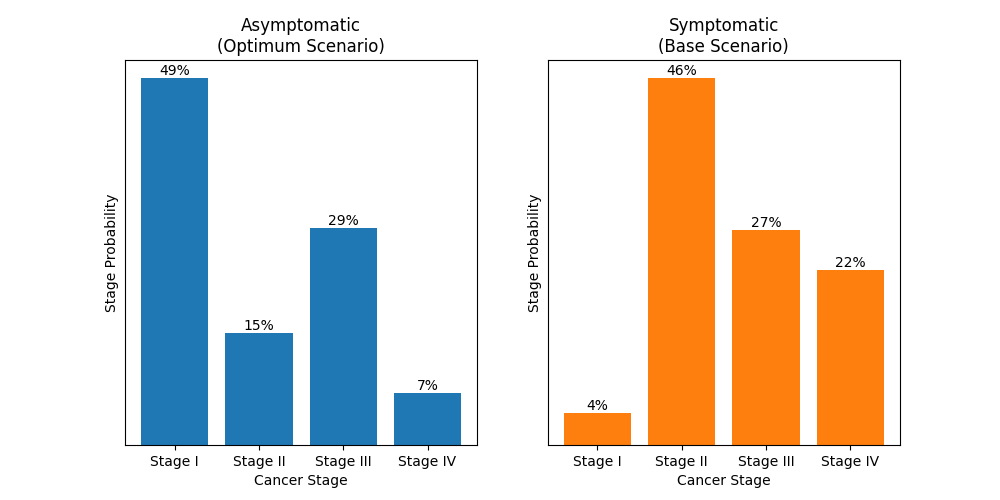
\includegraphics[scale=0.55]{images/cancer_stage_probability.png}
    \caption{Cancer Stage Probability}
    \label{fig:cancer_stage_probability}
\end{figure}
\end{center}

An important part of the model is based on the study by van Rossum et al. \cite{van_rossum_earlier_2009}. This study presents data on the stage probability distribution of CRC depending on whether it was detected asymptomatically or symptomatically, as shown in Figure \ref{fig:cancer_stage_probability}. Therefore, in a scenario where all CRC cases are detected asymptomatically, the CRC stage distribution should look like the graph on the left, and in the default case, in which all CRC cases are detected symptomatically, the CRC stage distribution should look like the graph on the right.

\subsection{Data collection}
\label{data_collection}

The MiCSS simulation model maintains three key data tables to support comprehensive analysis.

The first table, called the Census, records the population distribution by age. This allows the model to track demographic shifts and monitor age-specific data throughout the simulation.

The second table, Population Data, includes various health and demographic metrics: the total population, births, deaths, the number of individuals aged 50 to 75, the number of individuals with cancer, screening data (number screened, true positives, false negatives), and counts of asymptomatic and symptomatic detections. It also tracks treatments by cancer stage and records years gained, broken down into healthy years, disability-free years, and DALYs (disability-adjusted life years) gained.

The third table, Costs Data, details the financial aspects of the model. It tracks expenditures on FITs, colonoscopies, and total cancer treatment costs, including a breakdown of costs by cancer stage. This table provides insight into the economic impact of screening and treatment strategies within the simulation.

Using these data tables, the MiCSS model supports detailed cost-effectiveness analyses, enabling informed decisions on screening strategy policies.

\subsection{Model Specifics}

\subsubsection{Source of Cost Parameters}
For the MiCSS model, three primary costs were essential: the cost of FITs, colonoscopy procedures, and CRC treatments by stage.

The cost of conducting a FIT test was sourced from a private clinic in Chile that provided this screening service, ensuring a realistic price point within the region \cite{noauthor_aranceles_nodate-1}. For colonoscopies, data was obtained from three private clinics in Chile, with an average cost calculated to represent the expense accurately \cite{noauthor_aranceles_nodate,noauthor_aranceles_nodate-1,noauthor_aranceles_nodate-2}.

However, treatment costs for CRC patients segmented by stage of diagnosis were not available from Chilean sources. The Chilean GES (Garant\'ias Expl\'icitas en Salud) system defines a reference tariff for CRC surgery and reconstruction of approximately 3,755,430 CLP (3,968 USD) \cite{noauthor_superintendencia_2024}, but does not publish stage-specific total treatment costs including chemotherapy, follow-up, and supportive care. To overcome this limitation, the MiCSS model utilized data from a study by Mar et al. conducted in the Basque public healthcare system, which provides a comprehensive breakdown of lifetime treatment costs by cancer stage \cite{mar_cost_2017}. This is a recognized proxy in the literature for settings lacking local stage-specific cost data \cite{luengo-fernandez_economic_2013}. The Basque and Chilean healthcare systems share structural similarities as universal public health systems, and the costs were adjusted for inflation to 2023 CLP values. Future iterations should incorporate local cost data as it becomes available.

\subsubsection{Source of Benefit Parameters}

In the MiCSS model, the benefits of CRC screening are derived from early detection of asymptomatic cases. When an individual is detected with CRC in an asymptomatic stage, the model recalculates their life expectancy. Initially, life expectancy is based on a symptomatic stage, but an asymptomatic detection(often occurring at an earlier stage) results in a more favorable prognosis. The difference between the two calculations is recorded as ``years gained''. 

This process is similarly applied to other health metrics such as ``healthy years gained'', ``disability free years gained'' and ``Disability Adjusted Life Years(DALY) gained''. These metrics provide a comprehensive view of the screening's impact on both quantity and quality of life, showcasing the broader benefits of detecting CRC at earlier stages. All life expectancy data utilized in these calculations comes from a 2012 study from Soerjomataram et al. \cite{soerjomataram_most_2012}.

\newpage
\subsubsection{Model Parameters}
MiCSS includes a wide range of fixed parameters that can and should be updated as new information about CRC care becomes available. The parameters for the simulation are summarized in Table \ref{table:micss_model_default_parameters}:

\begin{table}[h]
\centering
\begin{tabularx}{\textwidth}{|X|X|X|}
\hline
\textbf{Description}         & \textbf{Value/s}  & \textbf{Source and Assumptions} \\ \hline
Starting year       & 2023   & Year of the Registered Population Data \\ \hline
Number of years     & 20     & Criteria of the researcher \\ \hline
Starting Registered Population & By age from 0 to 110 & Provided by the Southern Metropolitan Public Healthcare System (SMPHS) \\ \hline
Registrations per year & --Age 0: ND (9000, 500) & Calibrated to maintain population \\
                       & --Between Ages 1 and 8: ND (3200, 300) & \\
                       & --Between Ages 21 and 30: ND (1800, 300) & \\ \hline
Cohort Life Expectancies by Gender & By age from 0 to 119 and year from 1900 to 2095 & US Social Security Website \cite{noauthor_social_2024} \\ \hline
CRC Treatment Costs & --Stage I: 8,080.18 USD & Study by Mar et al. \cite{mar_cost_2017} \\
                    & --Stage II: 11,932.57 USD & \\
                    & --Stage III: 12,222.35 USD & \\
                    & --Stage IV: 47,985.18 USD & \\ \hline
FIT Cost & 6.2 USD & Price from UC Christus clinic \cite{noauthor_aranceles_nodate-1} \\ \hline
Colonoscopy Cost & 444.84 USD & Average Price from three Clinics \cite{noauthor_aranceles_nodate,noauthor_aranceles_nodate-1,noauthor_aranceles_nodate-2} \\ \hline
Age Interval of Screening & 50-75 & Most Common Age Interval in Europe \cite{navarro_colorectal_2017} \\ \hline
Frequency of Screening & Biennial & Recommended Frequency by the American College of Physicians \cite{qaseem_screening_2019} \\ \hline
CRC Lifetime Risk & 4.2\% & American Cancer Society \cite{noauthor_colorectal_nodate-1} \\ \hline
CRC Stage Distribution & --Symptomatic: I 4\%, II 46\%, III 27\%, IV 22\% & Study by van Rossum et al. \cite{van_rossum_earlier_2009} \\
                       & --Asymptomatic: I 49\%, II 15\%, III 29\%, IV 7\% & \\ \hline
Symptomatic Discovery Age Expectancy & Intervals of 5 from Ages 1 to 85+ & From US Cancer Statistics \cite{noauthor_uscs_2024} \\ \hline
Screenable Sojourn Time & Intervals by Age from 0 to 80+ & Study by Brenner et al. \cite{brenner_sojourn_2011} \\ \hline
CRC Life Expectancies (LE) & Normal LE, Healthy LE, and Disability-Free LE by sex, age, and stage from Ages 0 to 120 by Interpolation & Study by Soerjomataram et al. \cite{soerjomataram_most_2012} \\ \hline
FIT Performance & Sensitivity: 79\%, Specificity: 94\% & Meta Study by Lee et al. \cite{lee_accuracy_2014} \\ \hline
Polypectomy Prevention Rate & 52\% & Systematic review by Zhang et al. \cite{zhang_colonoscopic_2020} \\ \hline
Screening Adherence & 0\%, 5\%, 10\%, 15\%, 20\%, 40\%, 60\%, 80\% & Common Population Adherences \cite{navarro_colorectal_2017} \\ \hline
\end{tabularx}
\caption{MiCSS Model Default Parameters}
\label{table:micss_model_default_parameters}
\end{table}

\subsection{Model Transparency and Validation}

According to the Good Research Practices report by ISPOR and SMDM Task Force-7, trust and confidence in healthcare models require two complementary approaches: transparency and validation \cite{eddy_model_2012}. The report defines five types of validation---face validity, verification, cross validity, external validity, and predictive validity---each with distinct methods, strengths, and limitations. This section systematically addresses each type as applied to MiCSS.

The model's transparency is ensured by making all code, input data, and simulation outputs publicly available in a repository. The use of Python---one of the most widely used programming languages---ensures accessibility for anyone with basic programming knowledge.

\subsubsection{Face Validity}

Face validity was assessed through ongoing collaboration with three clinical experts: Dr.\ Francisco L\'opez Costner, Dr.\ Laura Itriago, and Dr.\ Francisco \'Alvarez. These physicians helped the modeler understand the medical aspects of colorectal cancer---natural history, the adenoma-carcinoma sequence, screening modalities (FIT and colonoscopy), test performance characteristics, treatment pathways by stage, and the Chilean healthcare context---so that the model could be constructed on a sound clinical foundation. Once the model was producing results, the experts reviewed the simulation outputs (CRC incidence rates, stage distributions, screening resource utilization, cost estimates, and DALY gains) and qualified them as reasonable given their clinical experience. A structured face validity checklist documenting what was reviewed and the experts' assessments is available in the repository.

\subsubsection{Verification (Internal Validity)}

Verification confirms that the code correctly implements the conceptual model. An automated test suite was developed using \texttt{pytest}, comprising two categories of tests:

\begin{itemize}
    \item \textbf{Extreme-value tests:} The model was run with boundary parameters to confirm expected behavior. With 0\% CRC prevalence, zero cancers and zero treatments were observed. With 0\% FIT sensitivity, zero true positives occurred. With 100\% FIT specificity, zero false positives occurred. With an impossible screening age range, zero FITs and colonoscopies were recorded. These tests confirm that the screening logic, cancer assignment, and cost calculations respond correctly to extreme inputs.
    \item \textbf{Conservation tests:} For each simulated year, the population count was verified to satisfy $P_{t+1} = P_t + \text{Births}_t - \text{Deaths}_t$. No person's age fell below 0 or exceeded 120 at any point during the simulation.
    \item \textbf{Consistency tests:} With perfect FIT sensitivity, every true positive results in either an asymptomatic treatment or a polypectomy. Cancer deaths are correctly tracked even after treatment through a persistent flag.
\end{itemize}

All 15 verification tests pass consistently across multiple runs.

\subsubsection{Cross Validity}

Cross validity compares model results against other models analyzing the same problem. The most established CRC screening microsimulation models are MISCAN-Colon, SimCRC, and CRC-SPIN, used jointly by CISNET to inform the USPSTF 2021 screening recommendations \cite{knudsen_colorectal_2021}.

Two complementary comparisons were performed. First, an \textbf{open-population comparison} used the standard MiCSS 200-year simulation (biennial FIT, ages 50--75, 80\% adherence). Metrics were reported both per 1,000 total population and per 1,000 screening-eligible population (ages 50--75), alongside life-years gained (LYG) to enable direct comparison with CISNET's primary outcome. When normalized to the eligible population, FIT utilization (399 per 1,000 per year) closely matched the CISNET annualized rate (371 per 1,000 per year), validating the screening frequency logic.

Second, a \textbf{closed-cohort comparison} followed 1,000 individuals from age 40 to death---matching the CISNET study design---with and without biennial FIT screening at 100\% adherence. This eliminates the denominator mismatch inherent in open-population comparisons. The closed-cohort results showed FIT utilization of 12,898 per 1,000 lifetime (vs.\ CISNET's 13,000---a 99.2\% match) and 18 CRC deaths averted per 1,000 (vs.\ CISNET's 5--8). The higher deaths averted reflects the polypectomy mechanism, which effectively cures 52\% of screening-detected cancers. LYG per 1,000 (57 vs.\ CISNET's 270--330) remains lower because the current LYG metric only captures gains from asymptomatic-to-symptomatic stage shifts, not the full life extension from polypectomy-prevented deaths. A detailed cross-validation comparison table and the closed-cohort benchmarking script are available in the repository.

\subsubsection{External Validity}

External validity compares model results against real-world observed data. Model outputs at 0\% screening adherence (the natural history baseline) were compared against Chilean epidemiological data:

\begin{itemize}
    \item \textbf{CRC incidence:} According to GLOBOCAN 2022, Chile had 6,778 new CRC cases in a population of 19.25 million \cite{ferlay_globocan_2024}. The MiCSS model simulates approximately 1.12 million individuals with a lifetime CRC risk of 4.2\%. Scaling model outputs to the national population yields approximately 8,805 annual cases, an overestimation of roughly 30\%. This likely reflects the use of a US-based lifetime CRC risk (4.2\%, from the American Cancer Society) that may exceed Chile's actual population risk.
    \item \textbf{CRC mortality:} GLOBOCAN 2022 reports 3,330 CRC deaths for Chile. The model's cancer death counts, when scaled nationally, yield approximately 6,977 deaths---an overestimation of roughly 110\%. This larger gap suggests that the cancer-specific life expectancy parameters may be too pessimistic, and that the model does not yet distinguish cancer-specific mortality from competing causes of death in cancer patients.
    \item \textbf{Stage distribution:} At 0\% adherence (symptomatic detection only), the model's stage distribution at diagnosis closely matches observed data: Stage I 3.8\% (observed 4.0\%), Stage II 46.1\% (46.0\%), Stage III 26.4\% (27.0\%), Stage IV 23.7\% (22.0\%), all within 2 percentage points of the distribution reported by van Rossum et al.\ (2009) \cite{van_rossum_earlier_2009}.
\end{itemize}

The stage distribution provides strong support for the model's screening logic and cancer assignment. The incidence and mortality overestimation warrant further investigation; formal quantitative calibration against Chilean cancer registry age-specific incidence curves and the use of Chile-specific lifetime CRC risk data are planned for a future iteration.

\subsubsection{Predictive Validity}

Predictive validity compares model predictions against prospectively observed events collected after the model was built. MiCSS was developed in 2023--2024 with a simulation starting year of 2023. As Chilean national cancer registry data for 2025--2026 become available, the model's 2--3 year projections of CRC incidence and screening resource utilization can be compared against observed values. A framework script for this comparison is included in the repository and will be populated with observed data as they are published.

\subsection{Implementation in Python}

One of the primary goals of this project was to develop a CRC screening model using entirely open source software, specifically the Python programming language. This choice was made to ensure both transparency and reproducibility of results. The code is fully accessible in a public repository, inviting others to use and verify the model.

Simulations were executed on a MacBook Air with an M1 chip. The duration varied by scenario count and simulation length. For the default run of 8 adherence scenarios over 20 years, the first scenario completed in 24 seconds, with all scenarios finishing in 192 seconds. In a longer simulation spanning 200 years, the first scenario took 257 seconds, with all completing in 37 minutes.

In the 200-year simulations, the population varied from 1,120,000 to 1,220,000 individuals. Over these extended periods of time, approximately 2.75 million people entered and left the simulation.

\newpage
\section{Results}

The results presented in this section were directly made with the information of the tables described in subsection \ref{data_collection}.

\subsection{Screening Efficacy}

\begin{center}
\begin{figure}[H]
    \centering
    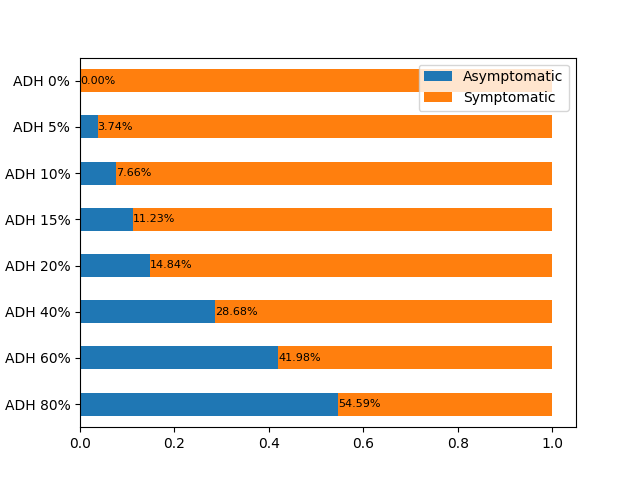
\includegraphics[scale=0.8]{images/screening_efficacy_by_adherence.png}
    \caption{Screening Efficacy by Adherence in the MiCSS model}
    \label{fig:screening_efficacy}
\end{figure}
\end{center}

The bar chart in Figure \ref{fig:screening_efficacy} shows the percentage of cases that are being diagnosed asymptomatically. With the default parameters, asymptomatic treatments constitute approximately three-quarters of the population's adherence to screening protocols.

In the 60\% adherence scenario, around 4 out of 10 patients will have their CRC stage determined by the asymptomatic distribution, while the other 6 will be categorized according to the symptomatic distribution. Both distributions are illustrated in Figure \ref{fig:cancer_stage_probability}.

\subsection{CRC Stage Distribution}

\begin{center}
\begin{figure}[H]
    \centering
    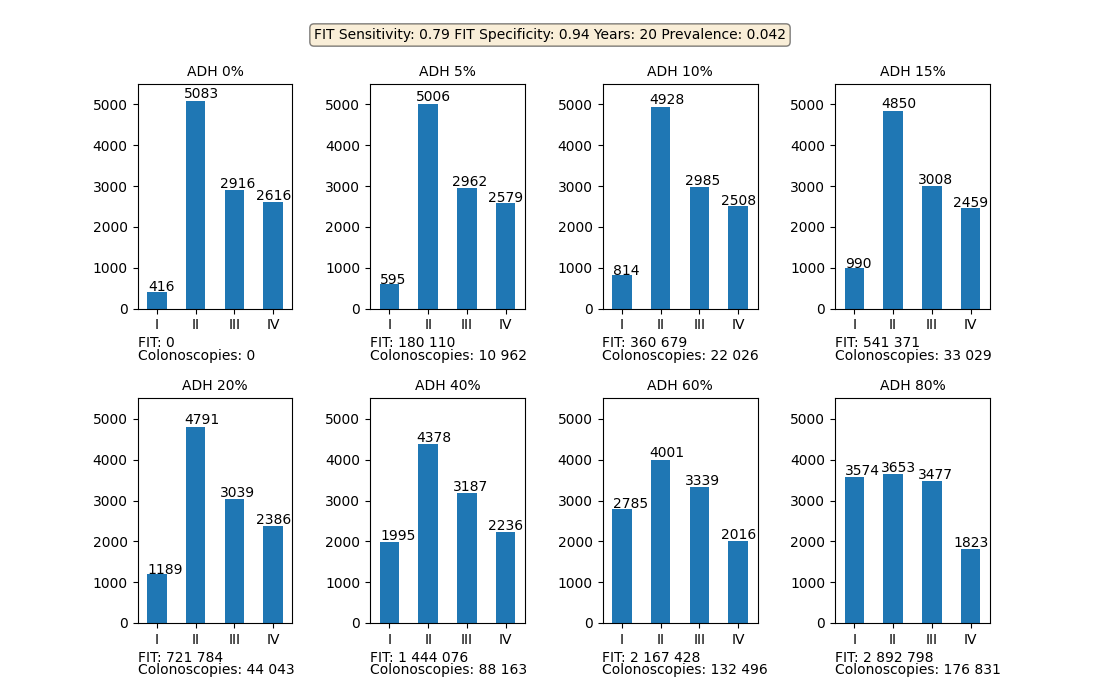
\includegraphics[scale=0.5]{images/treatments_by_adherence.png}
    \caption{CRC Stage Distribution by Adherence in the MiCSS model}
    \label{fig:crc_stage_distribution}
\end{figure}
\end{center}

Figure \ref{fig:crc_stage_distribution} depicts the shift towards earlier stages of CRC treatment as adherence rates increase. Additionally, the demand for resources, FITs and colonoscopies, rises over the 20-year period with higher adherence to screening protocols.

According to Navarro et al. \cite{navarro_colorectal_2017}, in the countries where CRC screening policies exist, the population adherence to them ranges from 16\% to 68\%. In 15\% and 60\% scenarios, the public healthcare system of the southern district of Santiago would need to perform between 26,512 to 106,179 FITs and 1,651 to 6,625 colonoscopies each year.

\subsection{Costs}

%\begin{center}
\begin{figure}[H]
    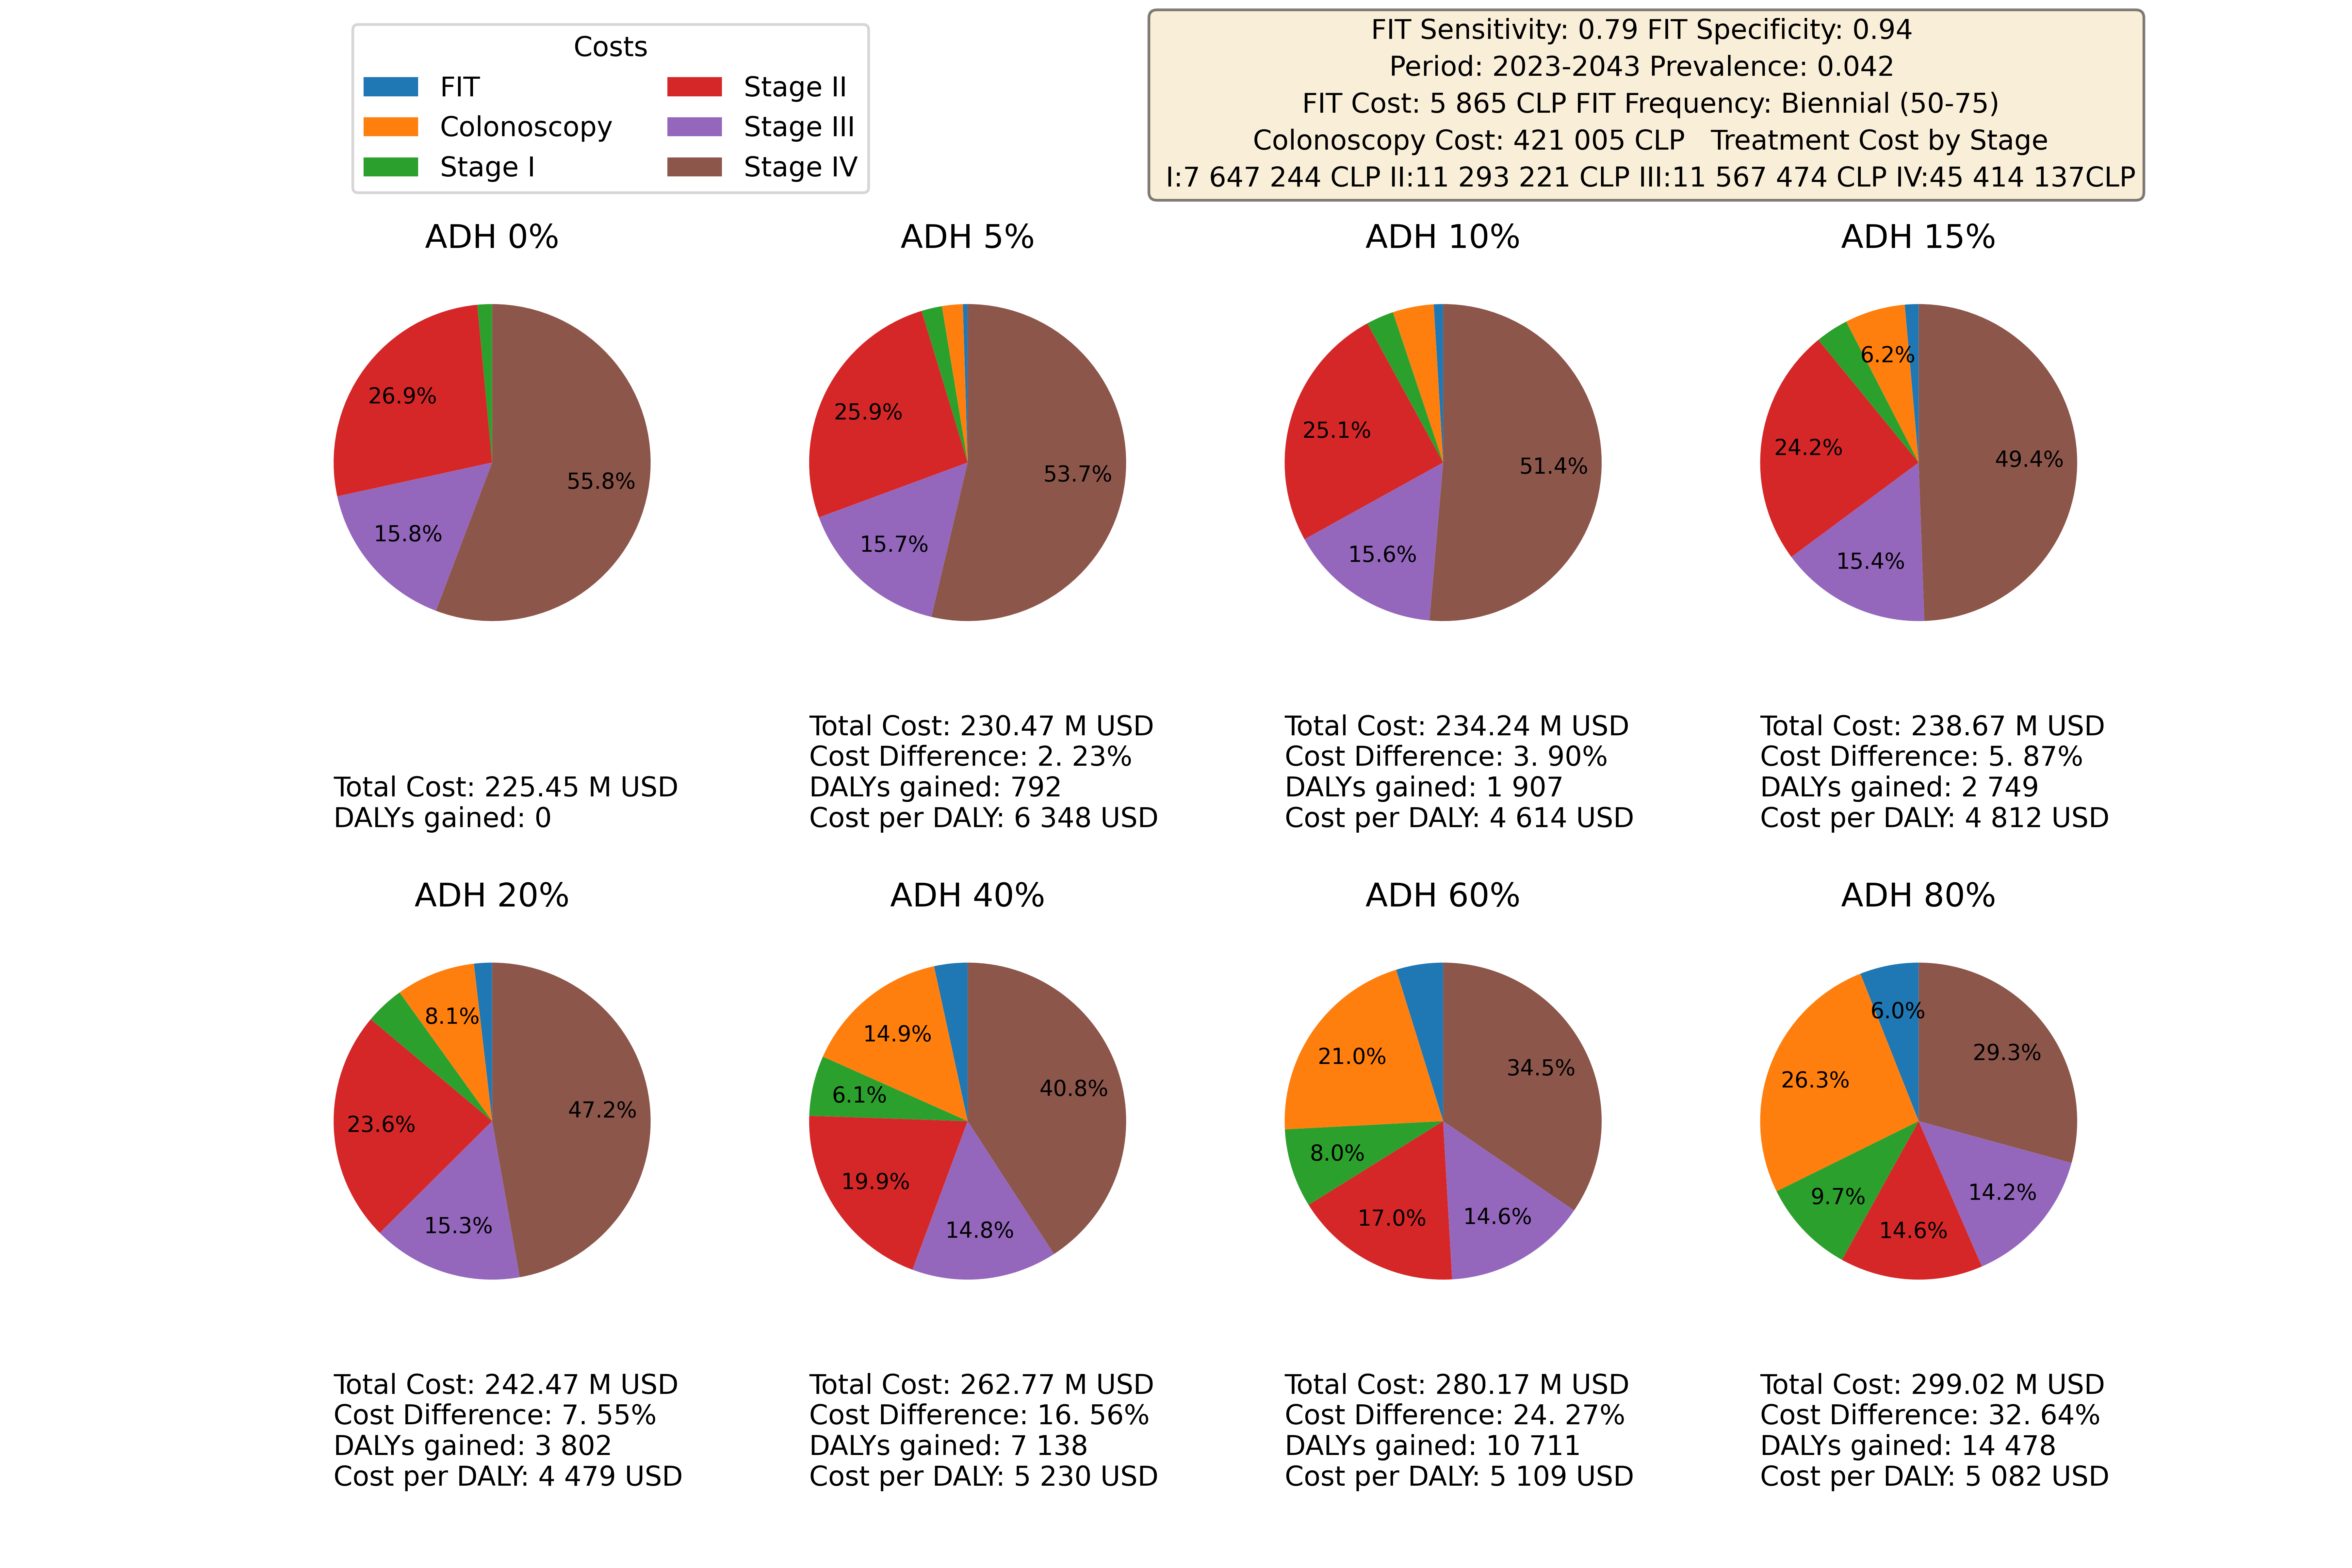
\includegraphics[scale=0.45, left]{images/costs_by_adherence_usd.png}
    \caption{CRC Costs by Adherence in the MiCSS model}
    \label{fig:costs_by_adherence}
\end{figure}
%\end{center}

Figure \ref{fig:costs_by_adherence} shows that as adherence rates increase, more monetary resources are allocated to FITs and colonoscopies, while spending on late-stage treatments decreases. Although overall costs rise with the implementation of the screening strategy, the costs of screening procedures are partially offset by the reduced costs associated with treating CRC at earlier stages and a significant number of disability-adjusted life years (DALYs) are gained. As depicted in Figure \ref{fig:costs_by_adherence}, the cost per DALY gained ranges from 4,479 USD to 6,348 USD, depending on the adherence rate.

According to the WHO-CHOICE framework \cite{noauthor_who-choice_2024}, an intervention is considered ``highly cost-effective'' when the cost per DALY averted is below one times the national GDP per capita, and ``cost-effective'' when below three times \cite{hutubessy_generalized_2003}. Chile's GDP per capita in 2024 was approximately 16,710 USD \cite{noauthor_world_bank_chile_2024}. The cost per DALY gained from biennial FIT screening in this model (4,479--6,348 USD) falls well below the 1$\times$ GDP per capita threshold, indicating that the screening strategy would be classified as \textbf{highly cost-effective} across all adherence levels studied.

In the extreme scenario of 80\% adherence, overall spending would increase by 32.6\%, but 54.6\% of CRC cases would be detected asymptomatically and 14,478 DALYs will have been gained.

\subsection{Deterministic Sensitivity Analysis}

To assess the robustness of the cost-effectiveness results, one-way deterministic sensitivity analyses were conducted by varying key model parameters while holding all others at their default values. The parameters varied and their impact on the cost per DALY gained are summarized in Table \ref{table:sensitivity_analysis}.

\begin{table}[H]
\centering
\begin{tabularx}{\textwidth}{|X|X|X|X|}
\hline
\textbf{Parameter} & \textbf{Range Tested} & \textbf{Cost/DALY Range (USD)} & \textbf{Impact} \\ \hline
FIT Sensitivity & 0.73 -- 0.85 & Minimal change ($<$1\%) & Low \\ \hline
FIT Specificity & 0.92 -- 0.96 & $\pm$8\% total cost & High \\ \hline
Colonoscopy Cost & 333,190 -- 504,205 CLP & $\pm$5\% total cost & Moderate \\ \hline
Screening Frequency & Annual -- Quinquennial & $\pm$25\% total cost & High \\ \hline
Screening Age Interval & 35--90 to 60--75 & $\pm$35\% DALYs gained & High \\ \hline
\end{tabularx}
\caption{One-Way Deterministic Sensitivity Analysis Results}
\label{table:sensitivity_analysis}
\end{table}

The analysis reveals that the cost per DALY gained remains below the 1$\times$ GDP per capita threshold (16,710 USD) across all parameter variations tested, indicating that the screening strategy is robust to parameter uncertainty. FIT specificity and screening frequency are the most influential parameters: a 2\% change in specificity shifts total costs by approximately 8\%, while moving from biennial to annual screening increases costs by approximately 25\%. In contrast, FIT sensitivity has minimal impact on overall cost-effectiveness. These findings suggest that efforts to improve test specificity and optimize screening frequency would yield the greatest policy returns.

\subsection{Probabilistic Sensitivity Analysis}

To complement the deterministic analysis, a probabilistic sensitivity analysis (PSA) was conducted by simultaneously sampling all key parameters from probability distributions across 1,000 iterations. FIT sensitivity and specificity were drawn from Beta distributions, treatment and screening costs from Gamma distributions, and CRC lifetime risk from a Beta distribution. Each iteration ran both a screening scenario (15\% adherence) and a no-screening baseline over the full 20-year horizon, computing incremental costs and incremental DALYs averted.

Table \ref{table:psa_results} summarizes the PSA results. Across 1,000 iterations, the mean incremental cost of screening was 4,570 million CLP (4,829 USD), with incremental DALYs gained averaging 1,264. The mean ICER was 3.65 million CLP per DALY averted (~3,858 USD/DALY). Notably, the 2.5th percentile of incremental cost was negative ($-$3,754 million CLP), indicating that in some parameter draws screening is cost-saving---treatment cost savings from polypectomy and early detection exceed screening costs.

\begin{table}[H]
\centering
\begin{tabularx}{\textwidth}{|X|X|X|X|X|}
\hline
\textbf{Metric} & \textbf{Mean} & \textbf{Median} & \textbf{2.5th \%ile} & \textbf{97.5th \%ile} \\ \hline
Incremental Cost (M CLP) & 4,570 & 4,349 & $-$3,754 & 13,577 \\ \hline
Incremental DALYs & 1,264 & 1,263 & 1,087 & 1,439 \\ \hline
Incremental LYG & 1,360 & 1,360 & 1,168 & 1,540 \\ \hline
ICER (M CLP/DALY) & 3.65 & 3.46 & $-$2.83 & 10.85 \\ \hline
\end{tabularx}
\caption{Probabilistic Sensitivity Analysis Results (1,000 iterations, 15\% adherence)}
\label{table:psa_results}
\end{table}

The cost-effectiveness acceptability curve (CEAC) indicates that at a willingness-to-pay (WTP) threshold of 10 million CLP per DALY ($\approx$10,569 USD), screening is cost-effective in 96.1\% of iterations. At Chile's GDP per capita ($\approx$17 million CLP), the probability of cost-effectiveness exceeds 99\%. These results strongly reinforce the conclusion from the deterministic analysis: biennial FIT screening is robustly cost-effective across plausible parameter uncertainty.

\newpage
\section{Discussion}

This article introduces the MiCSS model, designed to assess the cost effectiveness of implementing colorectal cancer (CRC) screening policies. The model integrates key epidemiological aspects of the disease, including test sensitivity, specificity, and the period of viable asymptomatic detection. By analyzing costs, resource requirements, and expected benefits—while accounting for population adherence—the MiCSS model provides policymakers with a comprehensive framework to evaluate the financial and health implications of different screening strategies.

The natural history of CRC is represented in the model, and sources for the parameters are openly disclosed to invite scrutiny and validation. Using demographic data from the southern district of the Metropolitan Region of Chile, birth parameters were calibrated to reflect the country’s population growth trends. The model produced plausible results regarding CRC cases, detections, resource utilization, and associated benefits.

A systematic review by Smith et al. (2020) examined colorectal cancer screening models published between 2008 and 2019 \cite{smith_simulation_2020}. Among 43 studies identified, only six utilized microsimulation models. Of these, four relied on the MISCAN-Colon model \cite{loeve_miscan-colon_1999}, one combined MISCAN-Colon with the SimCRC model \cite{noauthor_simcrc_nodate}, and the other used Canada’s OncoSim model \cite{gauvreau_oncosim_2017}. None of these models are publicly accessible, and MISCAN-Colon, despite its prevalence, is implemented in Delphi. In 2024 this programming language has a low 0.05\% share on the PYPL Index, which measures language popularity based on Google tutorial searches, far behind Python's dominant 29.71\% \cite{noauthor_pypl_nodate}.

In contrast, the MiCSS model is the only CRC screening microsimulation openly available for public use. Developed in Python, one of today’s most widely used programming languages, it minimizes barriers for those seeking to understand and utilize its code. Additionally, all data and sources are provided alongside the model, ensuring maximum transparency and reproducibility. This openness allows researchers, policymakers, and stakeholders to validate results and assess the model's accuracy independently.

Like any simulation, MiCSS simplifies complex processes to provide insights into the costs and benefits of screening policies. Its current version assumes stability over time in several factors, such as procedure costs, population adherence, and disease incidence. As E.P. Box famously stated, ``All models are wrong, but some are useful'' \cite{box_robustness_1979}. While the MiCSS model makes simplifications to CRC natural history and care processes, it has proven effective in delivering valuable insights into the cost effectiveness of CRC screening strategies.

\subsection{Limitations}

Several limitations should be acknowledged. First, treatment costs were derived from the Basque public healthcare system rather than Chilean sources, as stage-specific cost data are not publicly available in Chile. Second, the model assumes stable costs, adherence, and disease incidence over time. Third, adherence is modeled as a lifetime binary attribute rather than a dynamic behavior that may change over time; per-round adherence probabilities would be more realistic. Fourth, while external validation against GLOBOCAN 2022 shows good agreement in stage distribution, the model overestimates CRC incidence by approximately 30\% and CRC mortality by approximately 110\% when compared against national figures. These gaps likely stem from the use of US-based lifetime CRC risk parameters and the lack of competing-cause mortality modeling. Fifth, while the model has been validated following the five-type framework of Eddy et al.\ (2012)---including face validity, verification, cross validity (both open-population and closed-cohort), and external validity---formal quantitative calibration against Chilean cancer registry age-specific incidence curves has not yet been performed, and predictive validity awaits prospective data. Sixth, the life-years gained (LYG) metric does not yet capture the full benefit of polypectomy-prevented deaths, which restores natural lifespan but whose gained years are not included in LYG totals. This contributes to the gap observed in cross-validation against CISNET models.

\section{Conclusion}

The MiCSS model is an open source microsimulation tool that uses the best publicly available data on colorectal cancer natural history, test characteristics, and treatment costs. It evaluates the costs and benefits of screening strategies considering an entire population, including the protective effect of screening-induced polypectomy. Both deterministic and probabilistic sensitivity analyses confirm that biennial FIT screening would be highly cost-effective in the southern district of Santiago, Chile, with a cost per DALY gained well below the WHO-CHOICE threshold of 1$\times$ GDP per capita. The PSA shows that screening is cost-effective in over 96\% of 1,000 iterations at a WTP threshold of 10 million CLP per DALY, and in some iterations screening is cost-saving.

Moving forward, the researchers plan to further calibrate and enhance the model as new data on CRC becomes available. Priorities include incorporating Chilean cancer registry data for formal quantitative calibration to address the observed incidence and mortality overestimation, counting life-years gained from polypectomy-prevented deaths to capture the full screening benefit, adding surveillance colonoscopies, and updating treatment costs with local data as they become available. The ultimate goal is for MiCSS to contribute meaningfully to health policy design and become a trusted resource in the field.

\section*{Acknowledgements}
The authors extend their gratitude to the Southern Metropolitan Health Service of Chile for suggesting the development of this colorectal cancer model. Special thanks to Dr. Francisco López Costner, Dr. Laura Itriago and Dr. Francisco Álvarez for their guidance on the natural history, screening and treatment of colorectal cancer.

This work is part of Tomás Álvarez's master’s thesis.

\section*{Data Availability}
The complete model code, input data, and simulation outputs are publicly available at \url{https://github.com/Tomasalvarez15/crc\_screening\_simulator}. All monetary values in the text were converted from Chilean Pesos (CLP) to US Dollars (USD) using the exchange rate 1 USD = 946.42 CLP, obtained from Bloomberg (USDCLP:CUR) on July 2, 2024.

\backmatter
\newpage

\bibliography{sn-bibliography}% common bib file
%% if required, the content of .bbl file can be included here once bbl is generated
%%\input sn-article.bbl


\end{document}
